\documentclass[12pt]{article}
\usepackage[utf8]{inputenc}
\usepackage[T1]{fontenc}
\usepackage{fontspec}
\usepackage{natbib}
\setmainfont{Times New Roman}
\newfontfamily\hackfont{Hack}
\usepackage{titlesec}
\usepackage{fancyhdr}
\usepackage{fancyvrb}
\usepackage{listings}
\usepackage{xcolor}
\usepackage{graphicx}
\usepackage{longtable}
\usepackage{caption}
\usepackage{hyperref}
\usepackage{setspace}
\usepackage{multirow}
\usepackage{array}
\usepackage{tikz}
\usepackage{geometry}
\usepackage{pdfpages}
\geometry{a4paper, margin=1in}
\hypersetup{colorlinks=true, linkcolor=blue, urlcolor=blue}
\renewcommand{\contentsname}{Table of Contents}

\pagestyle{fancy}
\fancyhf{} 							% Header Middle
\rhead{Lab Report}
\lhead{Technical Writing}
\rfoot{\thepage}

\begin{document}

\begin{titlepage}					% Cover Start
\begin{center}
    
\includegraphics[width=0.35\textwidth]{logo.png} \\
    \vspace{0.5cm}
    \textbf{\Huge \textcolor{teal}{NOTRE DAME} \textcolor{teal}{UNIVERSITY}} \\
    \vspace{0.5cm}
    \textbf{\Huge \textcolor{orange}{BANGLADESH}} \\
    
    \vspace{0.9cm}
    \textbf{\Huge \underline{Technical Writing Lab Report}} \\
    
    \vspace{1.5em}
    \begin{flushleft}
    	\textbf{\Large Course Code: CSE-3207} \\
		\vspace{0.3cm}        
        \textbf{\Large Course Title: Technical Writing Presentation} \\
        \vspace{0.3cm}
        \textbf{\Large Lab Task Topic: Referencing and Citation in LaTeX} \\        
    \end{flushleft}
    
    \vspace{1em}
    \begin{flushleft}
        \textbf{\Huge \textcolor{blue}{Submitted by:}} \\
        \vspace{0.3cm}
        \textbf{\Large Name: Istiak Alam} \\
        \vspace{0.3cm}
        \textbf{\Large ID: 0692230005101005} \\
		\vspace{0.3cm}        
        \textbf{\Large Batch: CSE-20} \\
        \vspace{0.5cm}
        \textbf{\Large Submission Date: }{\Large \textbf{\today}\par}
    \end{flushleft}
    \vfill
    \begin{flushleft}
        \textbf{\Huge \textcolor{blue}{Submitted to:}} \\
        \vspace{0.3cm}
        \textbf{\Large Md. Tahmid Hasan} \\
        \vspace{0.3cm}
        \textbf{\Large Lecturer,} \\
        \vspace{0.3cm}
        \textbf{\Large Notre Dame University Bangladesh}
    \end{flushleft}
\end{center}
\end{titlepage}						% Cover End

\tableofcontents
\thispagestyle{empty}
\clearpage
\pagenumbering{arabic}

\section{Lab Report-01}
\subsection{Making Document Article in Texmaker}
\textbf{ $\bullet$ Code in Texmaker :}
\begin{verbatim}
\documentclass{article}
\begin{document}
\title{Practice Lab-01 :}
\author{Istiak Alam}
\maketitle
In March 2006, Congress raised that ceiling an additional \$0.79 trillion 
to \$8.97 trillion, which is approximately 68\% of GDP. As of October 4, 
2008, the ``Emergency Economic Srabilization Act of 2008" raised the 
current debt ceiling to \$11.3 trillion.
\end{document}
\end{verbatim}
\textbf{\\ $\bullet$ Output in Texmaker :}
\begin{figure}[h!]
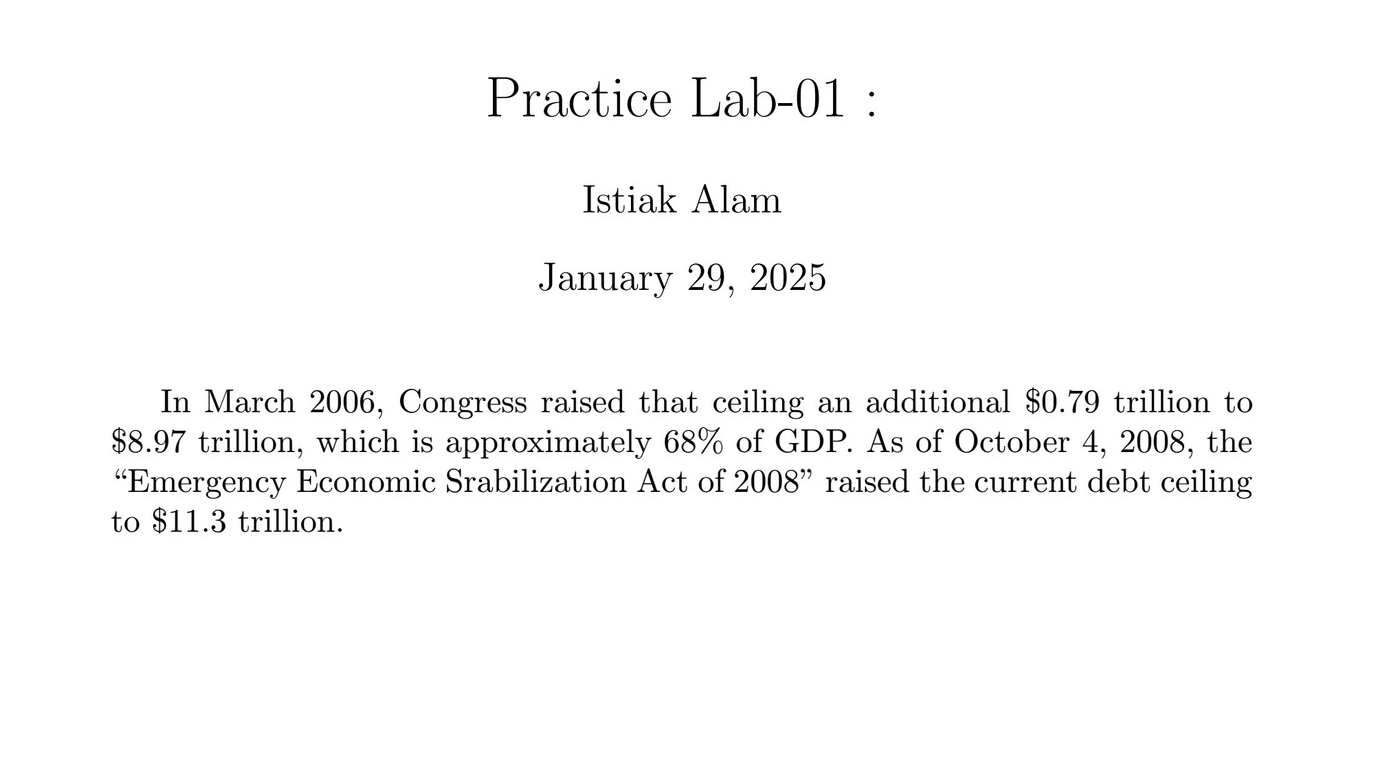
\includegraphics[width=1\textwidth]{lab1.png}
%\caption{\label{table}Output of the Article}
\end{figure}
\newpage
\section{Lab Report-02}
\subsection{Mathamatical Equation}
\textbf{ $\bullet$ Code in Texmaker :}
\begin{verbatim}
\documentclass{article}
\begin{document}
\title{Practice Lab-02 :}
\author{Istiak Alam}
\maketitle
\textbf{Mathamatical Equation:} \\
1. $\int k\ dx = kx + C$ \\
2. $\int x^n\ dx = \frac{1}{n+1}x^{n+1}+C,\ n \neq -1 $\\
3. $\int x^{-1}\ dx = \int \frac{1}{x}\ dx = ln|x|+C$ \\
4. $\int \frac{1}{ax+b}\ dx=\frac{1}{a}ln|ax+b|+C$ \\
5. $\int ln(x)\ dx = x ln(x) -x + C $ \\
6. $\int e^x\ dx = e^x + C$ \\
7. $\int cosx\ dx = sinx + C$ \\
8. $\int sinx\ dx = -cosx + C$ \\
9. $\int sec^2x\ dx = tanx + C$ \\
10. $\int secx\ tanx\ dx = secx + C$\\ \\
11. $\int cscx\ cotx\ dx = -cscx + C$ \\ \\
12. $\int csc^2x\ dx = -cotx + C$ \\ \\
13. $\int tanx\ dx = ln|secx| + C$ \\ \\
14. $\int secx\ dx = ln|secx+tanx| + C$ \\ \\
15. $\int \frac{1}{(a^2+u^2)}\ dx = \frac{1}{a}tan^{-1}
(\frac{u}{a})+C$ \\
16. $\int \frac{1}{\sqrt[]{a^2-u^2}}\ dx = 
sin^{-1}\frac{u}{a}+C$
\end{document}
\end{verbatim}
\newpage
\textbf{ $\bullet$ Output in Texmaker :}
\begin{figure}[h!]
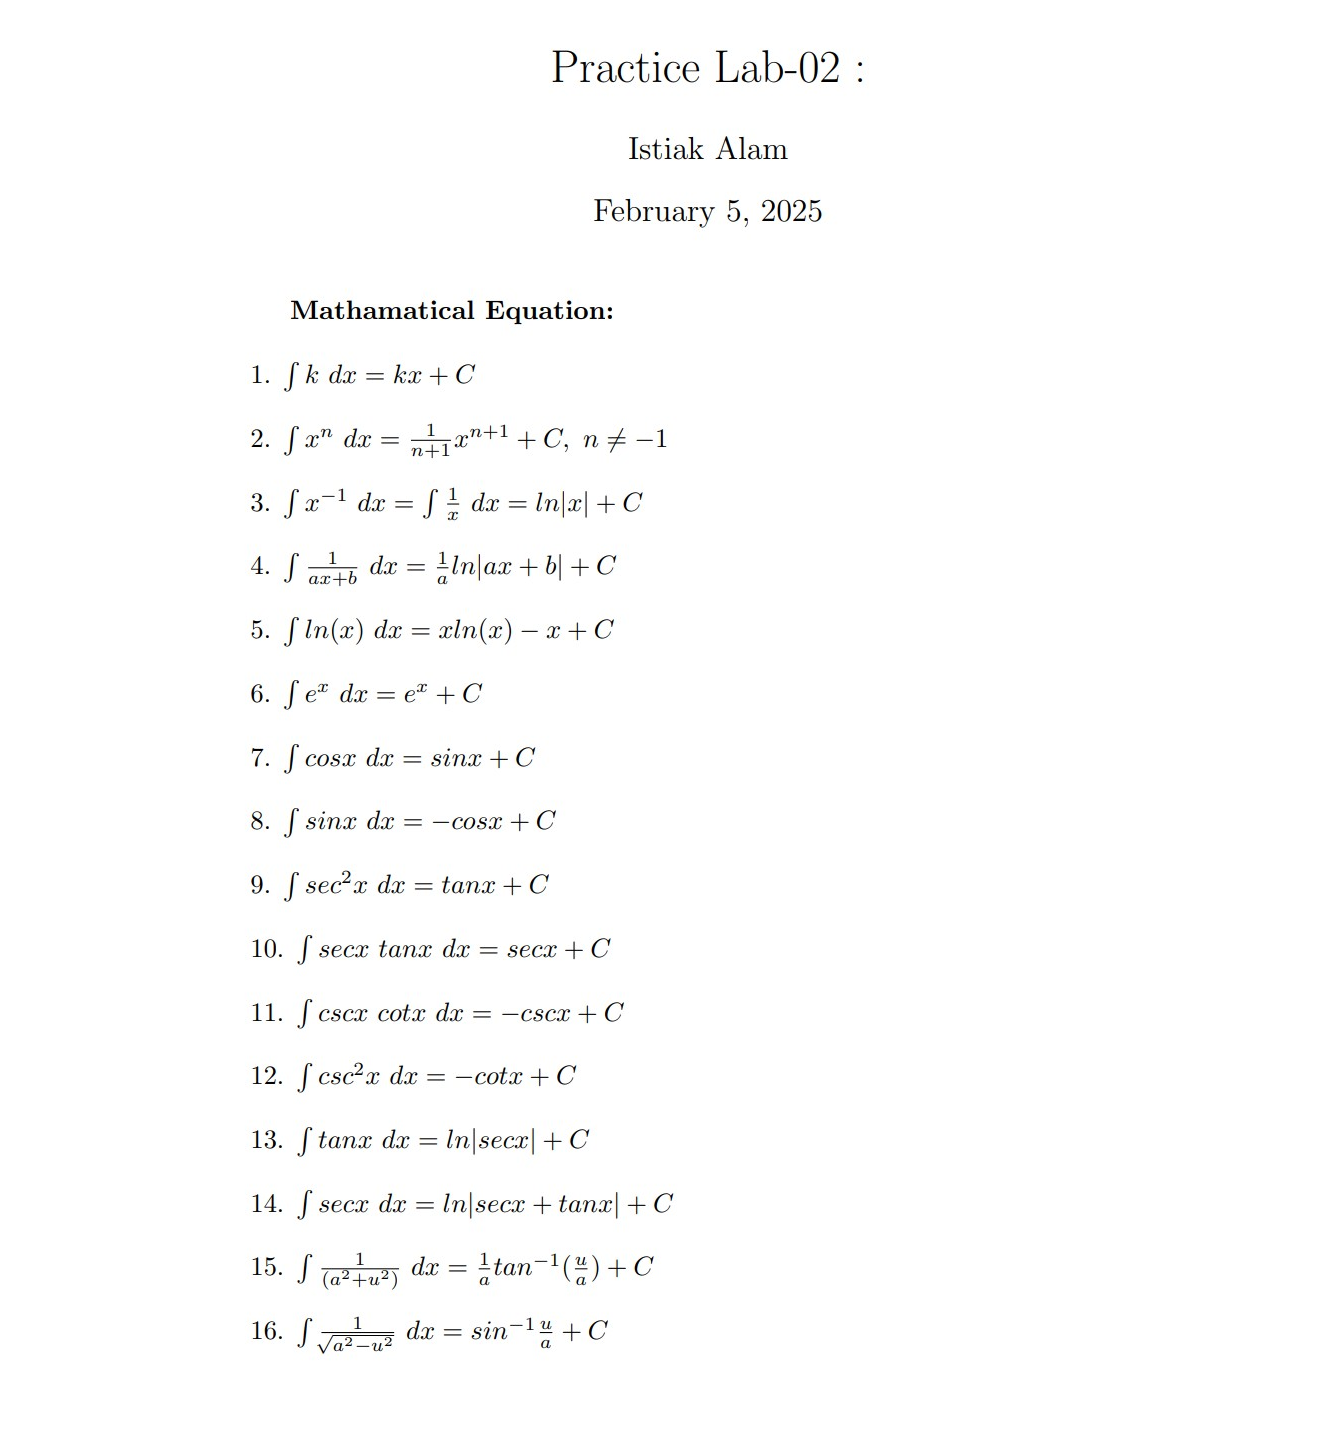
\includegraphics[width=1.1\textwidth]{lab2.png}
%\caption{\label{table}Output of the Article}
\end{figure}
\newpage
\section{Lab Report-03}
\subsection{Integral Equations}
\textbf{ $\bullet$ Code in Texmaker :}
\begin{verbatim}
\documentclass[13pt]{article}
\begin{document}
\title{Practice Lab-03 :}
\author{Istiak Alam}
\maketitle
\textbf{Integration Properies:} \\ \\
1. $\int^b_a\ cf(x)\ dx = c \int^b_a\ f(x)\ dx$
2. $\int^b_a\ f(x) \pm g(x)\ dx = \int^a_b\ f(x)\ dx \pm \int^a_b g(x)\ dx$
3. $\int^b_a\ f(x)\ dx = 0\ and \int^b_a\ f(x)\ dx = - \int^b_a f(x)\ dx $
4. $\int^b_a\ f(x)\ dx + \int^c_b f(x)\ dx = \int^c_a f(x)\ dx$
\end{document}
\end{verbatim}

\textbf{\\ $\bullet$ Output in Texmaker :}
\begin{figure}[h!]
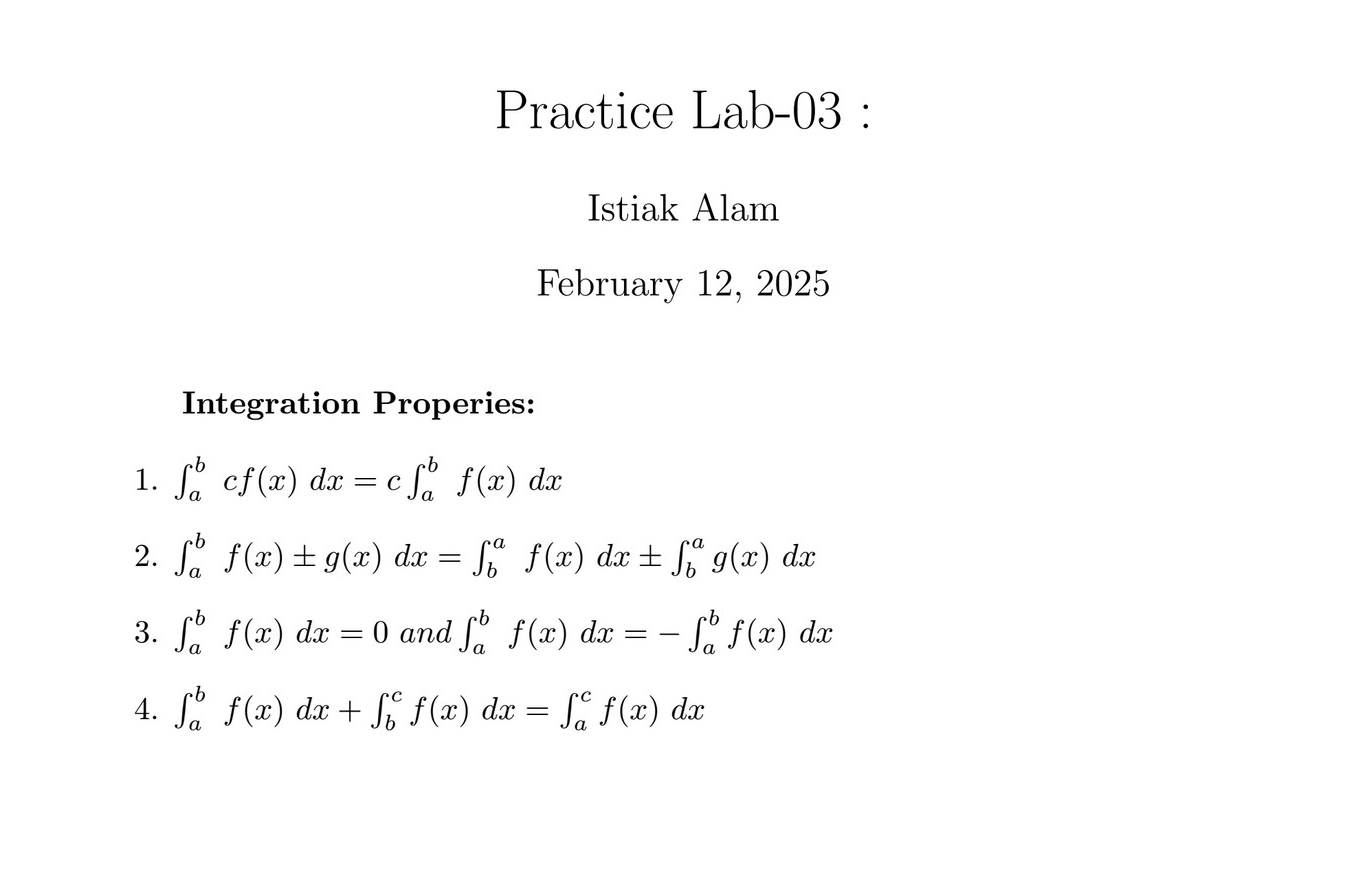
\includegraphics[width=1\textwidth]{lab3.png}
%\caption{\label{table}Output of the Article}
\end{figure}
\newpage
\section{Lab Report-04}
\subsection{Street Style `Chicken Roll' Recipe}
\textbf{ $\bullet$ Code in Texmaker :}
\begin{Verbatim}[fontsize=\footnotesize]
\documentclass[14pt]{article}
\begin{document}
\title{\underline{Lab Task-04} \\ Question-01 : Street Style `Chicken Roll' Recipe} 
\author{Istiak Alam | ID : 05}
\maketitle

\section{Ingredients of Chicken Roll}

\begin{enumerate}
    \item $\frac{1}{3}$ Cup and 2 and $\frac{1}{2}$ tablespoon chicken
    \item $\frac{1}{2}$ Medium tomato
    \item Red chilli powder as required
    \item 1 Tablespoon vegetable oil
    \item $\frac{1}{4}$ Cucumber
    \item $\frac{1}{4}$ Tablespoon coriander leaves
    \item $\frac{1}{2}$ Large onion
    \item 1 Medium green chilli
    \item 1 Pinch garam masala powder
    \item $\frac{1}{2}$ Lemon wedge
    \item $\frac{1}{2}$ Teaspoon tomato ketchup
    \item $\frac{1}{2}$ Tablespoon green chilli sauce
\end{enumerate}

\section{For Marination}
\begin{enumerate}
    \item $\frac{1}{4}$ teaspoon coriander powder
    \item Turmeric as required
    \item 1 pinch black pepper
    \item $\frac{1}{4}$ teaspoon garlic paste
    \item $\frac{1}{4}$ teaspoon cumin powder
    \item $\frac{1}{2}$ teaspoon low-fat yoghurt
    \item $\frac{1}{4}$ teaspoon ginger paste
\end{enumerate}

\section{For Dough}
\begin{enumerate}
    \item Salt as required
    \item $\frac{1}{4}$ tablespoon vegetable oil
    \item $\frac{1}{2}$ cup all-purpose flour
    \item $\frac{1}{4}$ cup water
\end{enumerate}

\section{Preparation}

\begin{itemize}
    \item For preparing this easy snack recipe, take a glass bowl and add coriander powder, 
    black pepper, garlic paste, cumin powder, low fat yoghurt, turmeric and ginger paste in it. 
    Mix well. Add the freshly washed chicken pieces in the bowl and marinate them with the 
    already added ingredients. Keep aside for minimum 1 hour or more.
\end{itemize}

\section{Cooking}
\begin{itemize}
    \item Now heat oil in a frying pan over moderate flame. Add sliced onions and saute them on
     medium flame until light brown in colour. Then add chopped tomatoes and cook for 2-3 minutes. 
     Then add the marinated chicken pieces. Mix well, cover and cook on low flame for 10 minutes. 
     Keep stirring in between. Add ½ cup of water.
    \item Cover and cook until the chicken is done, stir in between. If the chicken is drying too 
     much, sprinkle some more water. Once done add garam masala powder. Mix well and 
     remove from heat. Keep it aside.
\end{itemize}

\section{Preparing the Dough}
\begin{itemize}
    \item For the dough, mix well all purpose flower, vegetable oil and salt. Now add water 
     slowly and knead a very smooth dough. Make 3 or 4 equal sized balls out of it. On a lightly
     floured surface, roll out each ball into a round paratha (the thickness should be little 
     bit more than the regular chapatis or rotis).
\end{itemize}

\section{Cooking the Paratha}
\begin{itemize}
    \item Heat a tawa on moderate flame and cook the paratha one at a time. Flip and cook both 
    sides without oil first (cook for a minute in total), now add 1 tbsp oil for each side. 
    Flip and cook until light brown spot appears. Avoid too much flipping as the parathas may 
    get hard. Remove from heat and keep the parathas aside.
\end{itemize}

\section{Assembling the Roll}
\begin{itemize}
    \item Now on a hot paratha, arrange some cooked chicken pieces in a row (make this line little
     apart from the center). Drizzle some lemon juice all over the chicken pieces, garnish with 
     some sliced onions, cucumber and chopped coriander leaves. Add few drops of tomato ketchup
     and chili sauce.
    \item Roll the paratha firmly and wrap one half of the roll with tissue paper. Fold the bottom
     part of the tissue paper inside the roll. Your street style ‘Chicken Roll’ is ready to eat. 
     Enjoy!
\end{itemize}

\end{document}
\end{Verbatim}
\vfill
\textbf{ $\bullet$ Output in Texmaker :}
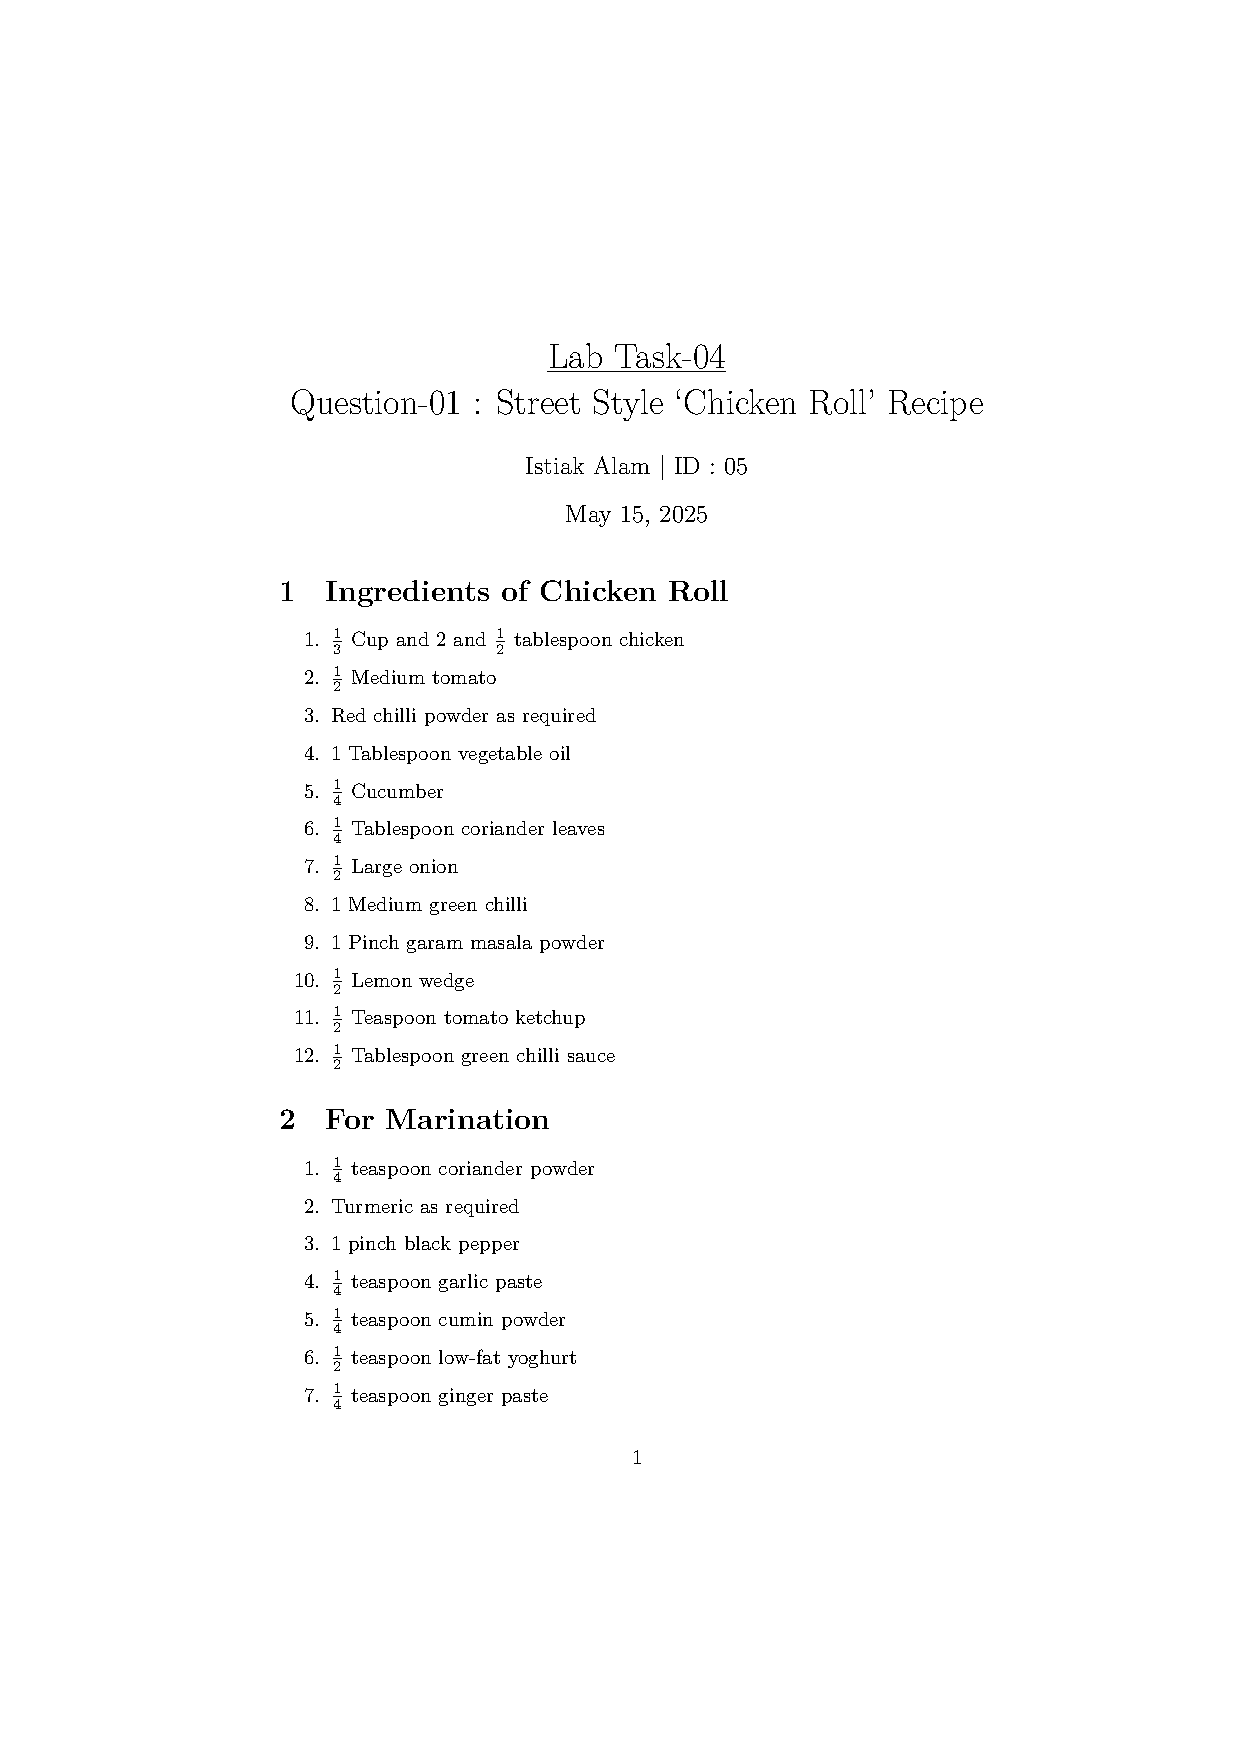
\includepdf[pages=-]{lab4.pdf}

\subsection{Gammy's Apple Pie}
\textbf{ $\bullet$ Code in Texmaker :}
\begin{Verbatim}[fontsize=\footnotesize]
\documentclass[14pt]{article}
\begin{document}
\title{\underline{Lab Task-04} \\ Question-02 : Recipe of Gammy's Apple Pie }
\author{Istiak Alam | ID : 05}
\maketitle

\section{Crust}
\begin{enumerate}
    \item 2 cups flour
    \item 1 tsp salt
    \item $\frac{3}{4}$ cup solid shortening (like Crisco)
    \item $\frac{1}{4}$ to $\frac{1}{2}$ cup ice water
\end{enumerate}

\subsection*{Preparation}
\begin{itemize}
\item Mix together the flour and the salt. Cut in the shortening until the pieces are pea-sized. 
Add $\frac{1}{4}$ to $\frac{1}{2}$ cup of the water and stir with a fork until the dough is moist 
enough to stick together but is not soggy.
\item Sprinkle your pastry cloth (or whatever you use) with flour. Divide the pie crust dough in 
slightly uneven halves. Form the larger of the two halves into a ball and place on the pastry cloth. 
Pat into a circle about five inches in diameter. Begin to roll out from the center outward with 
light strokes. Be sure your rolling pin is floured also.
\item Once the circle is about 7 inches in diameter, pick up the piece of dough, reflour underneath 
it and flip it over. This will ensure that there is enough flour to keep the dough from sticking. \\
(Note: If the dough is sticking too much, that means you put too much water in it. Add more flour. 
If the dough is crumbly and won't stick together at all, that means it needs more water.)
\item Resume rolling it out until you reach the size of your pie pan (usually 9 or 10 inches). 
At this point, you can roll out the edges, too. 
The idea is just to not have too much dough in the middle.
\item Once the dough is the proper size (Don't worry; it won't be even.), pick it up by rolling it 
around the rolling pin. Carefully transfer it to the pie pan doing your best to center it over the 
pan. Once you release it from the rolling pin, gently pat it in place in the pan, making sure there 
aren't any gaps between the dough and the inside edge of the plate. Trim the dough with a knife 
so that it is even with the edge of the pie pan. Throw the extra dough in the bowl with the 
remaining half.
\item At this point, you would add your fruit filling and then proceed with the top crust. The top 
crust is made virtually the same way; however, you would want it rolled out a little bigger than the 
bottom so that you have enough crust to flute. I flute by pinching the crust between my two index 
fingers and thumbs as though I was opening a change purse. Be sure to cut slits in the top crust 
for the steam to escape.
\end{itemize}

\section{Filling}
\begin{enumerate}
    \item 3-4 Granny Smith apples, peeled and sliced
    \item $\frac{1}{2}$ Cup brown sugar
    \item $\frac{1}{2}$ Cup granulated sugar
    \item $\frac{1}{2}$ Cup flour
    \item 1 tsp apple pie spice (or 1 tsp cinnamon and $\frac{1}{2}$ tsp nutmeg)
\end{enumerate}

\subsection*{Preparation}
\begin{itemize}
\item Line pie plate with unbaked pastry. Mix together the sugars, flour and spices. Pour 1/2 of 
this mixture into the pie plate, smoothing evenly across the bottom. Lay the apples in the crust, 
enough so that they reach the top of the plate but aren't mounded over it. Sprinkle the remaining 
flour mixture over the top of the apples. Sprinkle 1 tablespoon of lemon juice over the top, then 
dot with 1 tablespoon of butter. Add the top crust and cut slits for steam.	
\end{itemize}

\section{Baking Instructions}
\begin{itemize}
    \item Bake 15 minutes at 425°, then reduce heat to 350° and bake another hour. The trick with
     apple pie is to be sure and bake it long enough for the apples to be soft. I usually stick a 
     fork inside one of the slits to make sure, but an hour should be plenty. If the edge of the 
     crust starts to brown too much, cover it loosely with foil.
\end{itemize}
It's a good idea to set the pie on a cookie sheet in case the apples are particularly juicy and 
spill over into the oven. \\

\center Enjoy your homemade Gammy's Apple Pie!

\end{document}

\end{Verbatim}
\vfill
\textbf{ $\bullet$ Output in Texmaker :}
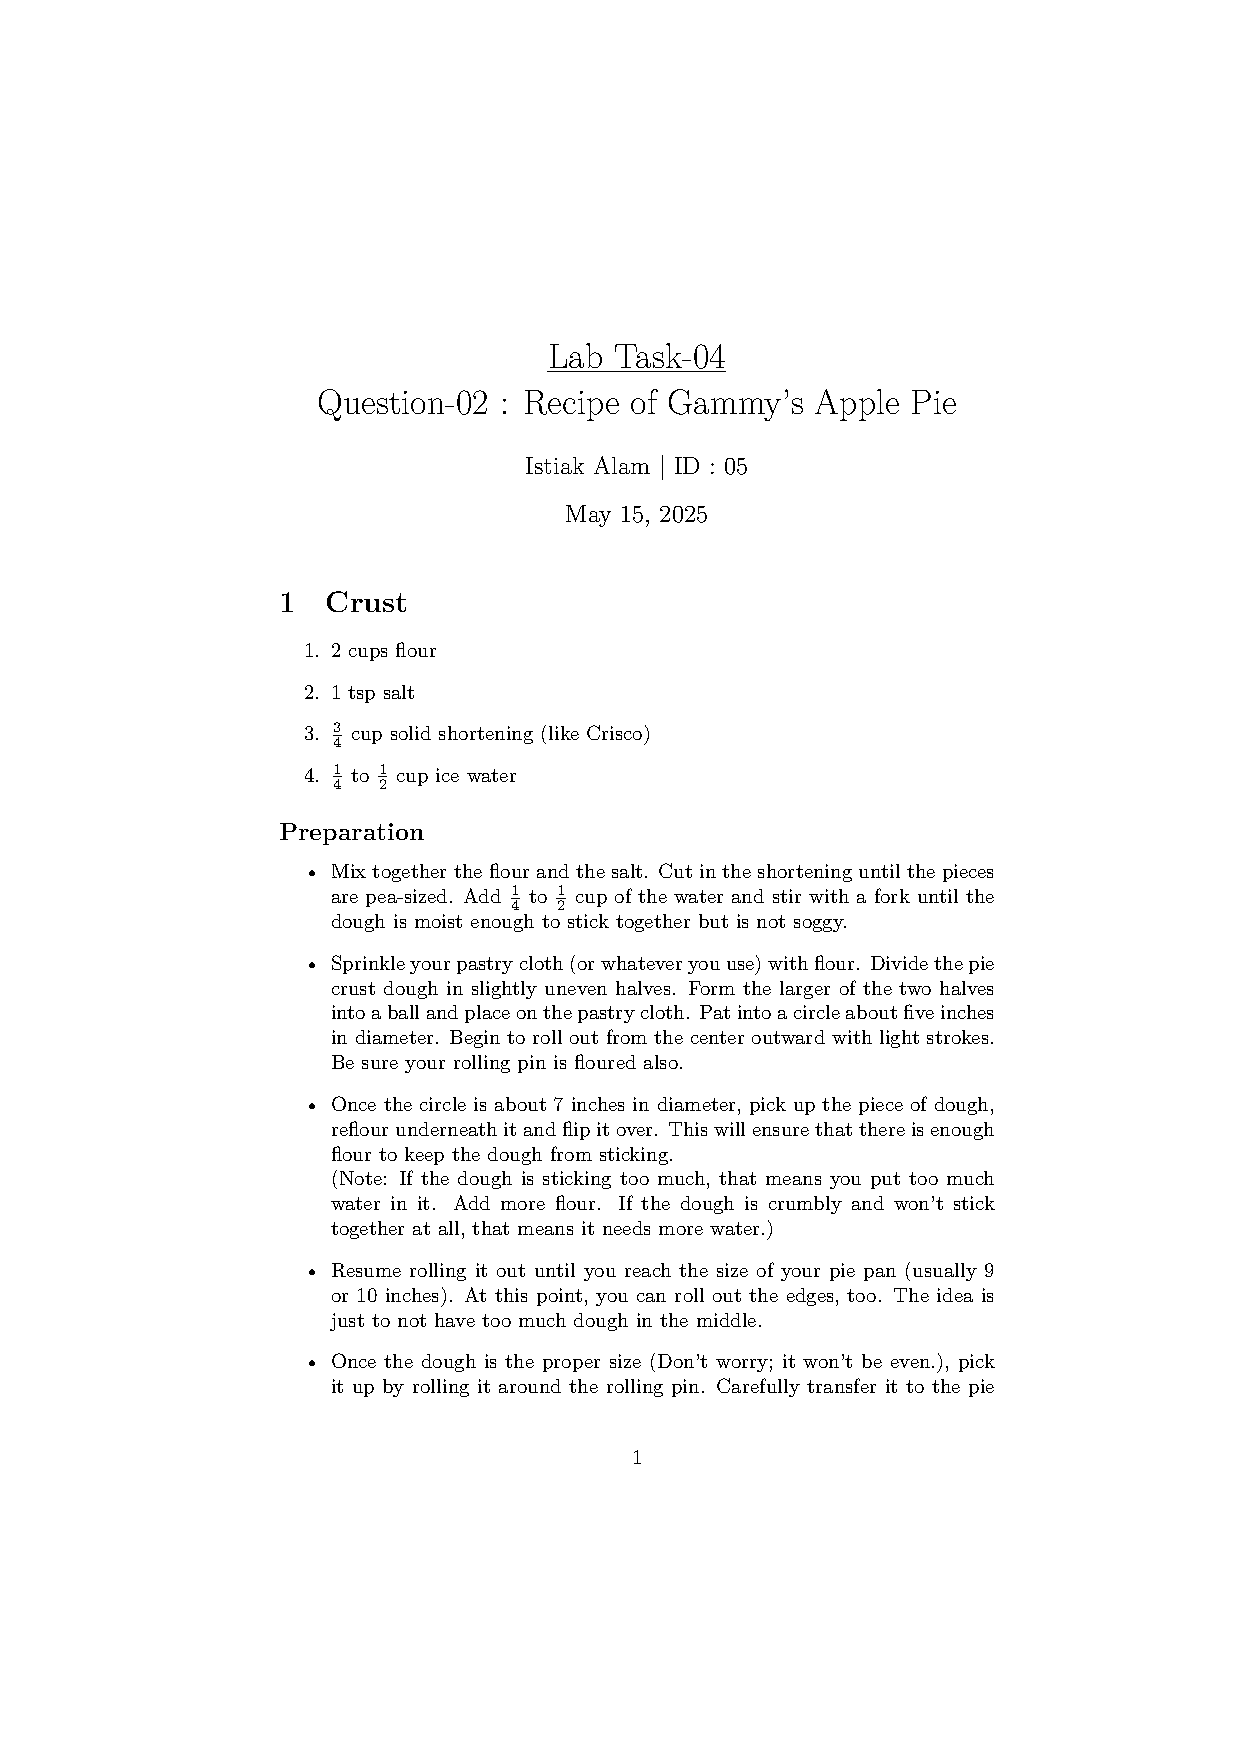
\includepdf[pages=-]{lab42.pdf}

\section{Lab Report-05}
\subsection{Packages}
\textbf{ $\bullet$ Code in Texmaker :}
\begin{Verbatim}
\documentclass[13pt]{article}
\usepackage{enumitem}
\usepackage{amsmath}
\begin{document}
\title{Practice Lab-05 : \\ Packages}
\author{Istiak Alam}
\maketitle
\begin{enumerate}[label=\Alph*.]
 \item 1/3 cup and 2 and 1/2 tablespoon chicken
 \item 1/2 medium tomato
 \item Red chilli powder as required
 \item 1 tablespoon vegetable oil
 \item 1/2 tablespoon green chilli sauce \\ \\
\end{enumerate}
With Equation Number
\begin{equation}
\Omega = \sum_{k=1}^{n} \omega_k
\end{equation}
Without Equation Number
\begin{equation*}
\Omega = \sum_{k=1}^{n} \omega_k \\ \\
\end{equation*}
\begin{equation*} %bad
min_{x,y} (1-x)^2 + 100(y-x^2)^2
\end{equation*}
\begin{equation*} %Good
\min_{x,y}{(1-x)^2+100(y-x^2)^2}
\end{equation*}
\begin{equation*}
\beta_i =
\frac{\operatorname{Cov}(R_i, R_m)}
 {\operatorname{Var}(R_m)}
\end{equation*}
\begin{align*}
(x+1)^3 &= (x+1)(x+1)(x+1) \\
 &= (x+1) (x^2 + 2x + 1) \\
 &= x^3 + 3x^2 + 3x + 1
\end{align*}
\end{document}

\end{Verbatim}
\vfill
\textbf{ $\bullet$ Output in Texmaker :}
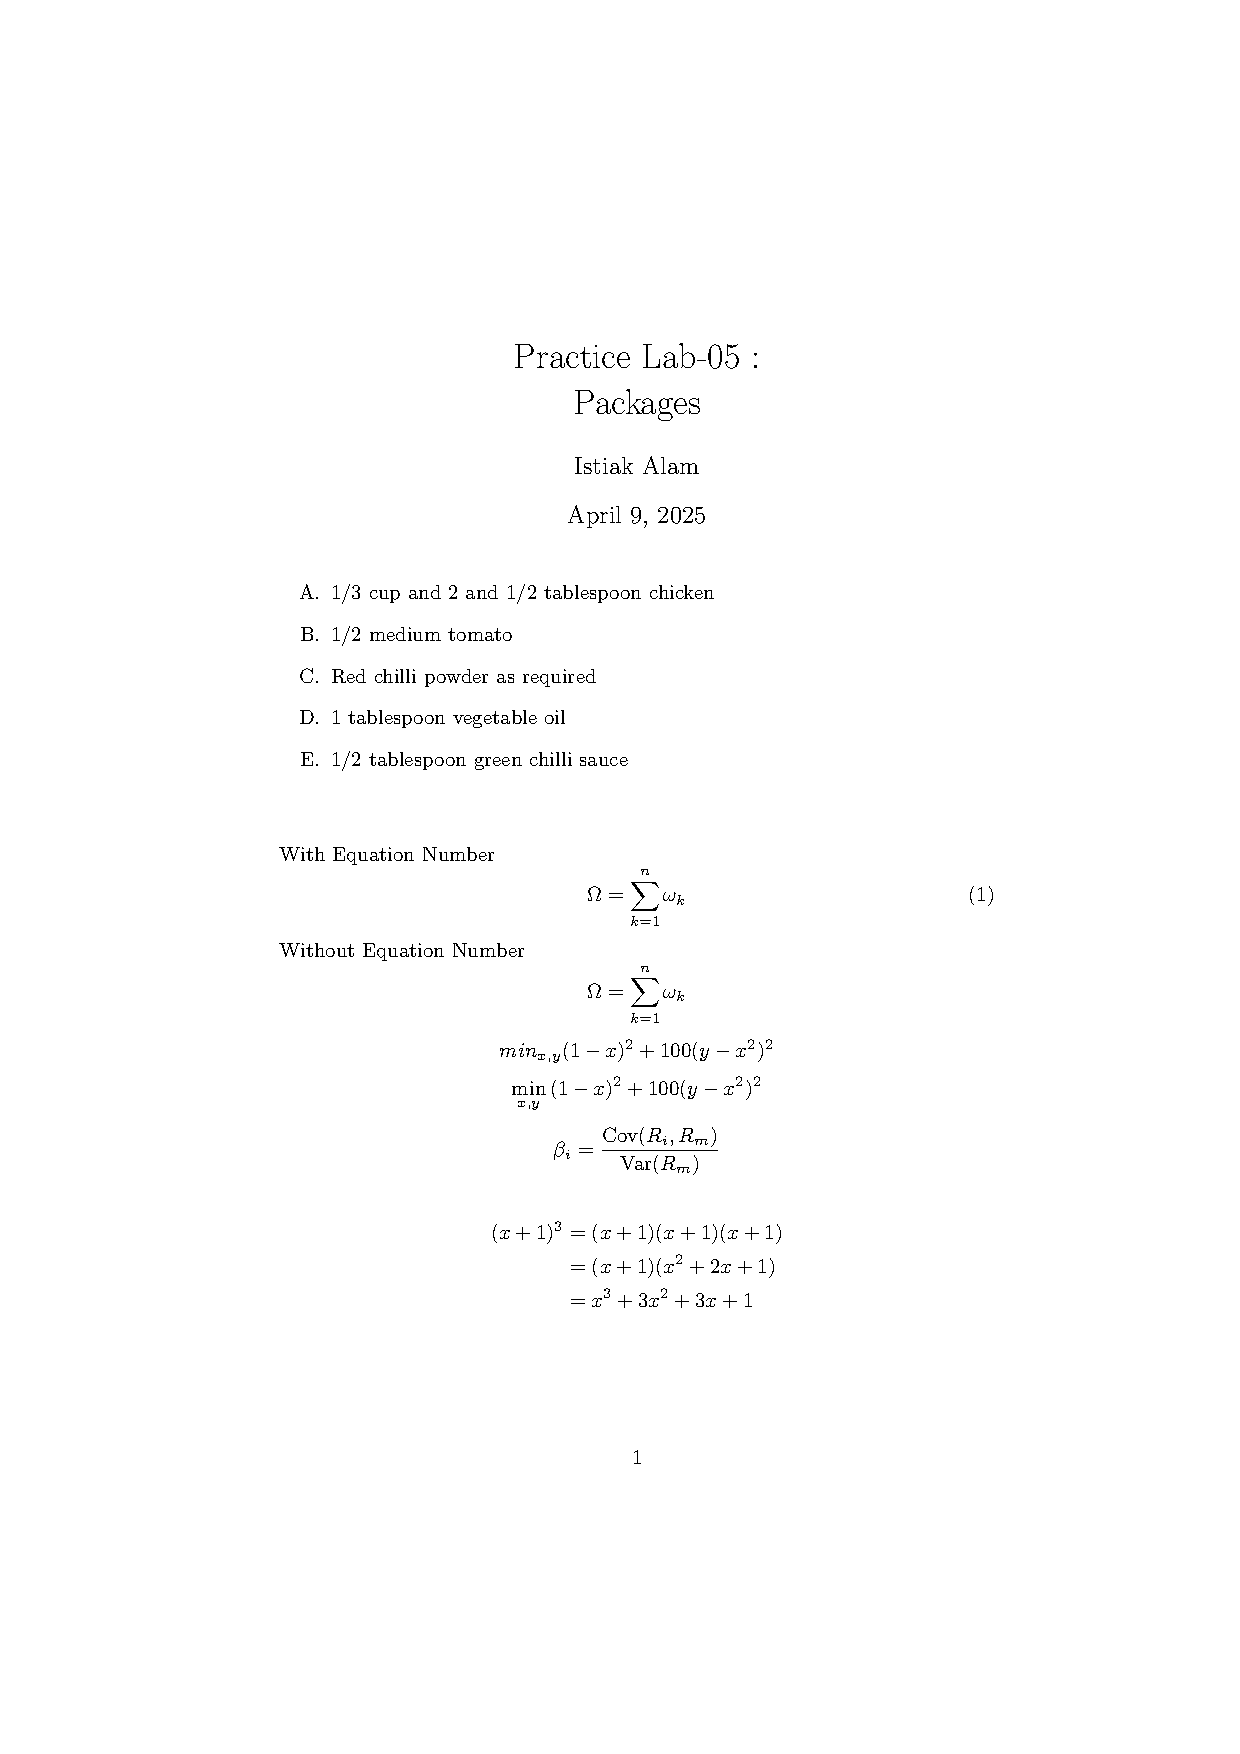
\includepdf[pages=-]{lab5.pdf}

\subsection{Typesetting Exercise}
\textbf{ $\bullet$ Code in Texmaker :}
\begin{Verbatim}[fontsize=\footnotesize]
\documentclass[13pt]{article}
\usepackage{amsmath}
\begin{document}
\title{Lab Task-05 : \\ Typesetting Exercise 2}
\author{Istiak Alam}
\maketitle
\section{Typeset in LaTex}
%\textbf{Typeset in LaTex}
Let $X_1,X_2,...,X_n$ be a sequence of independent and identically 
distributed random variables with E$[X_i]=\mu$ and Var$
[X_i]=\sigma^2<\infty$ \\
\begin{equation*}
S_n = \frac{1}{n} \sum^n_i X_i
\end{equation*}
donote their mean. then as $n$ approaches infinity, the random variables $
\sqrt{n}(S_n-\mu)$ converge in distribution to a normal $N(0,\sigma^2)$.
\end{document}
\end{Verbatim}

\textbf{\\ \\ $\bullet$ Output in Texmaker :}
\begin{figure}[h!]
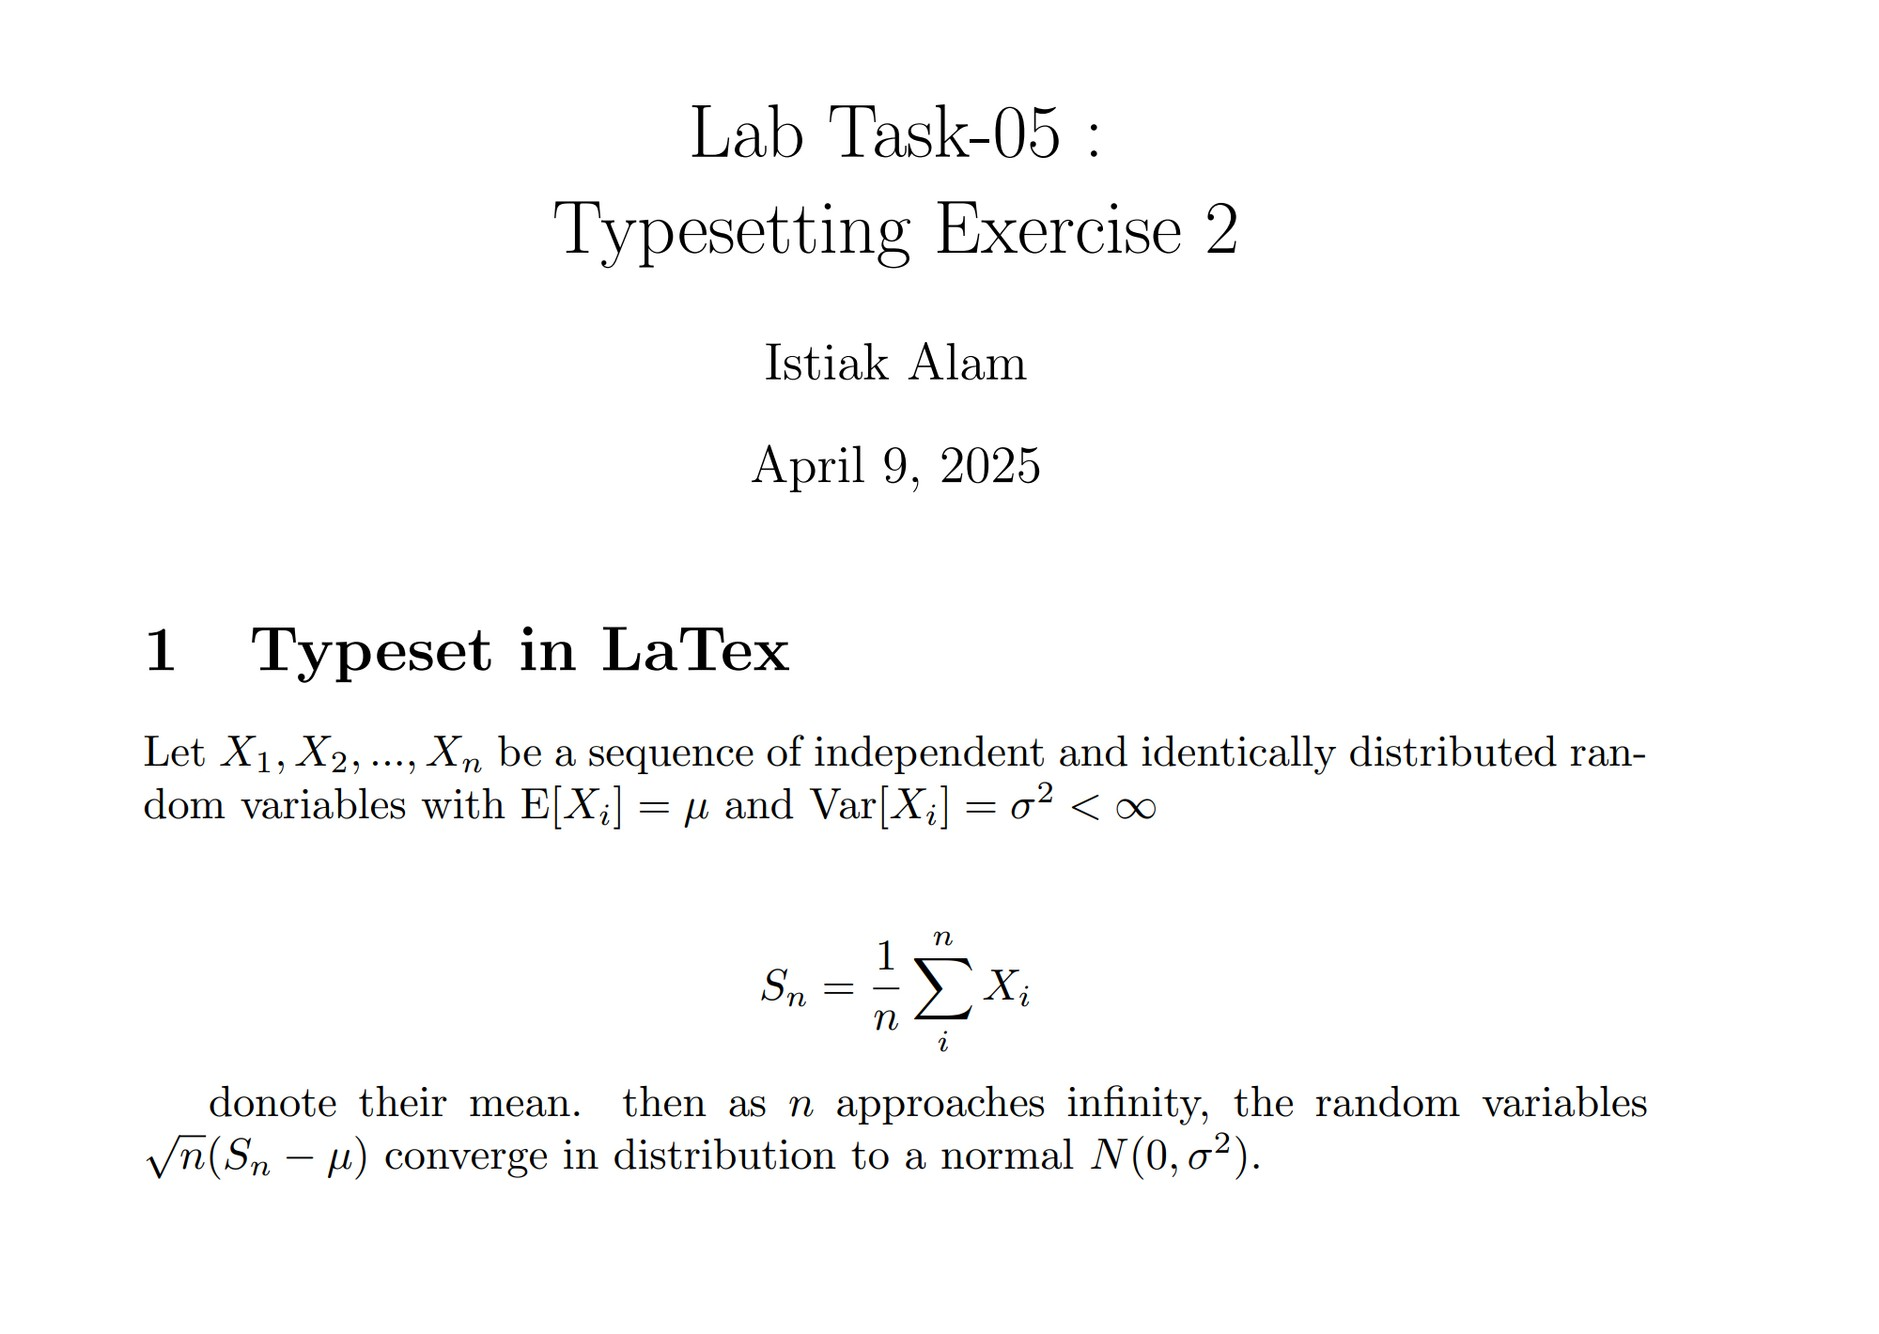
\includegraphics[width=1\textwidth]{lab5.png}
%\caption{\label{table}Output of the Article}
\end{figure}
\section{Lab Report-06}
\subsection{Structure Exercise in LaTeX}
\textbf{ $\bullet$ Code in Texmaker :}
\begin{Verbatim}[fontsize=\footnotesize]
\documentclass[12pt]{article}
\usepackage{amsmath}
\usepackage{geometry}
\geometry{margin=1in}
\title{The Relationship Between the UNIVAC\\Computer and Evolutionary Programming}
\author{Bob, Carol and Alice}
\date{February 20, 2014}
\begin{document}
\maketitle
\begin{abstract}
Many electrical engineers would agree that, had it not been for online algorithms, the 
evaluation of red-black trees might never have occurred. In our research, we demonstrate 
the significant unification of massive multiplayer online role-playing games and the 
location-identity split. We concentrate our efforts on demonstrating that reinforcement 
learning can be made peer-to-peer, autonomous, and cacheable.
\end{abstract}
\section{Introduction}
Many analysts would agree that, had it not been for DHCP, the improvement of erasure coding 
might never have occurred. The notion that hackers worldwide connect with low-energy algorithms
is often useful. LIVING explores flexible archetypes. Such a claim might seem unexpected but 
is supported by prior work in the field. The exploration of the location identity split would 
profoundly degrade metamorphic models.
The rest of this paper is organized as follows. In section 2, we describe the methodology used. 
In section 3, we conclude.
\section{Method}
Virtual methods are particularly practical when it comes to the understanding of journaling 
file systems. It should be noted that our heuristic is built on the principles of cryptography. 
Our approach is captured by the fundamental equation (1).
\begin{equation}
E = mc^3
\end{equation}
Nevertheless, certifiable configurations might not be the panacea that end users expected. 
Unfortunately, this approach is continuously encouraging. 
Certainly, we emphasize that our framework caches the investigation of neural networks. 
Thus, we argue not only that the infamous heterogeneous algorithm for the analysis of the 
UNIVAC computer by Williams and Suzuki is impossible, but that the same is true for object-
oriented languages.
\section{Conclusions}
Our contributions are threefold. To begin with, we concentrate our efforts on disproving that 
gigabit switches can be made random, authenticated, and modular. Continuing with this rationale, 
we motivate a distributed tool for constructing semaphores (LIVING), which we use to disconfirm 
that public private key pairs and the location-identity split can connect to realize this objective. 
Third, we confirm that A* search and sensor networks are never incompatible.
\end{document}
\end{Verbatim}
\vfill
\textbf{ $\bullet$ Output in Texmaker :}
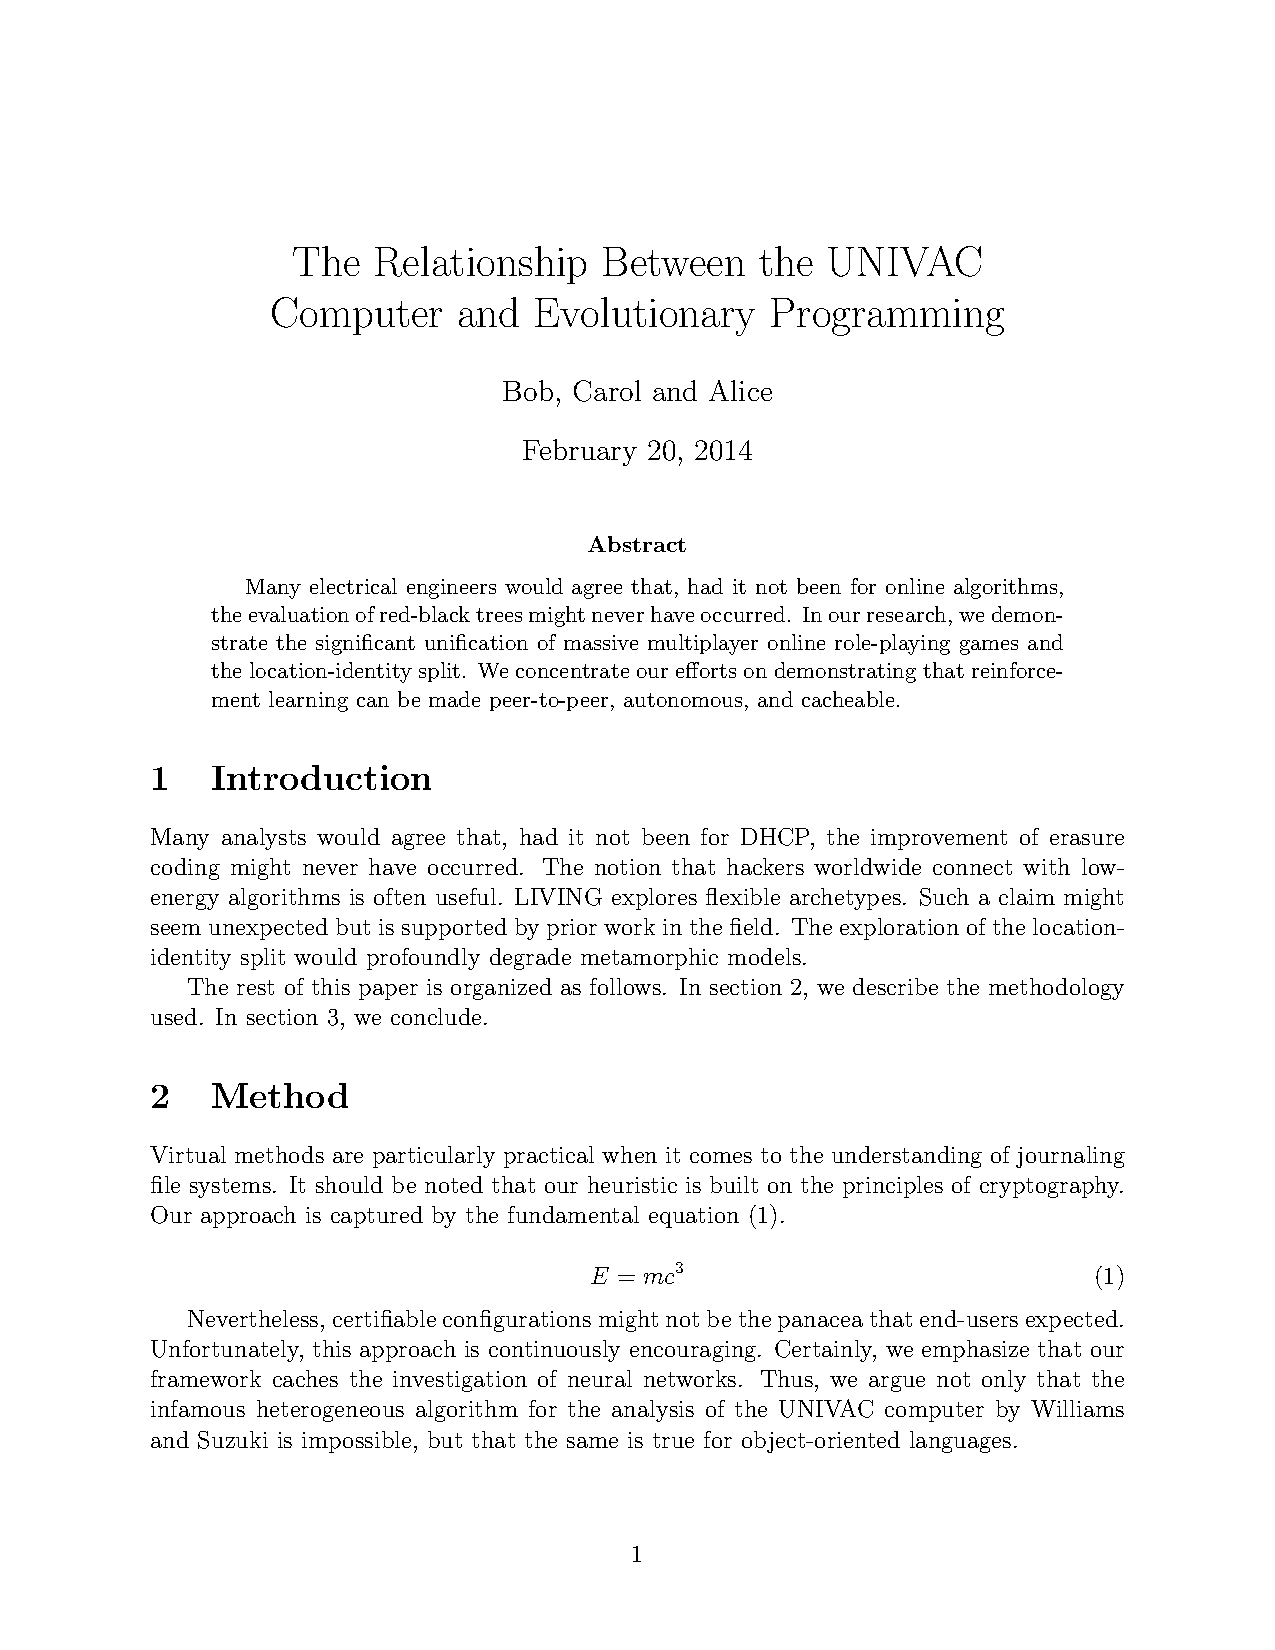
\includepdf[pages=-]{lab6.pdf}

\section{Lab Report-07}
\subsection{Table Formating in LaTaX}
\textbf{ $\bullet$ Code in Texmaker :}
\begin{Verbatim}[fontsize=\footnotesize]
\setlength{\extrarowheight}{20pt}
\begin{tabular}{cc}

 \setlength{\extrarowheight}{7pt}
\begin{tabular}{|c|c|c|c|}
\hline
A & \multicolumn{3}{c|}{C} \\
\hline
\multirow{2}{*}{B} & \multirow{2}{*}{D} & 
\multirow{2}{*}{E} & F \\
\cline{4-4}
 &  &  & G \\
\hline
\multicolumn{4}{|c|}{H} \\
\hline
\multicolumn{4}{|c|}{I} \\
\hline 
\end{tabular}  &

\noindent
\makebox[0pt][l]{
\hspace{-0.9cm}

\setlength{\extrarowheight}{12pt}
\begin{tabular}{|c|c|c|c|}
\hline
\multicolumn{2}{|c|}{P} & \multicolumn{2}{c|}{R} \\
\hline
\multicolumn{2}{|c|}{Q} & \multicolumn{2}{c|}{S} \\
\hline
T & V & X & \multirow{2}{*}{Z}\\
\cline{1-3}
U & W & Y &  \\
\hline
\end{tabular} } \\

\raisebox{2.85cm}{
\makebox[0pt][l]{
\hspace{-1.7cm}

 \setlength{\extrarowheight}{1.5pt}
\begin{tabular}{|c|c|c|c|}
\hline
\multirow{3}{*}{J} & \multirow{3}{*}{K} & 
\multirow{3}{*}{L} & M \\
\cline{4-4}
 &  &  & N \\
\cline{4-4}
 &  &  & O \\
\hline
\end{tabular} } } & 

\raisebox{2.2cm}{
\makebox[0pt][l]{
\hspace{-0.82cm}

\begin{tikzpicture}[scale=0.48]
    % Here I use a rectangle border
    \draw[thick] (0,0) rectangle (6,3);


    % Here is a diagonals
    \draw[thick] (0,0) -- (6,3);
    \draw[thick] (0,3) -- (6,0);

    % using node for text
    \node at (3,2.5) {THIS};
    \node at (1,1.5) {IS};
    \node at (5,1.5) {NOT};
    \node at (3,0.5) {EASY};
\end{tikzpicture} } } \\

\end{tabular}
\end{Verbatim}
\textbf{\\ $\bullet$ Output in Texmaker :}
\begin{figure}[h!]
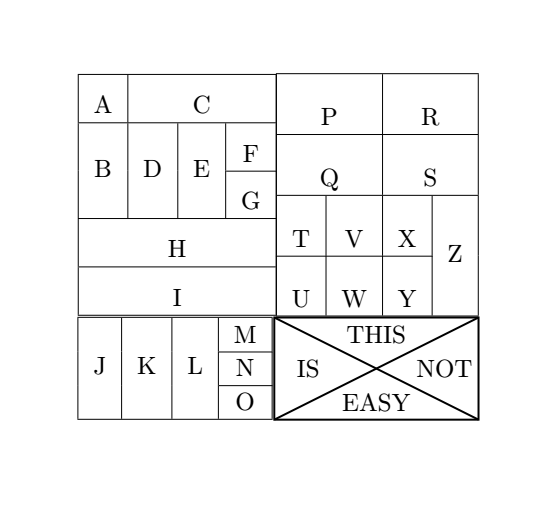
\includegraphics[width=0.9\textwidth]{lab7.png}
%\caption{\label{table}Output of the Article}
\end{figure}
\newpage

\section{Lab Report-08}
\subsection{Add Citations in LaTeX}
\textbf{ $\bullet$ Code in Texmaker :}
\subsubsection*{main.tex}
\begin{Verbatim}[fontsize=\footnotesize]
\documentclass{article}
\usepackage{natbib}
\begin{document}
Adding References in LaTeX File : \\
\citet{Brooks1997Methodology}
show that \ldots. Clearly,
all odd numbers are prime
\citep{Jacobson1999Towards}.
\bibliography{references}
% if `bib-example' is the name of
% your bib file
\bibliographystyle{plainnat}
% try changing to abbrvnat
\end{document}
\end{Verbatim}

\subsubsection*{references.bib}
\begin{Verbatim}[fontsize=\footnotesize]
@Article{Jacobson1999Towards,
author = {Van Jacobson},
title = {Towards the Analysis of Massive Multiplayer Online
Role-Playing Games},
journal = {Journal of Ubiquitous Information},
Month = jun,
Year = 1999,
Volume = 6,
Pages = {75--83}}
@InProceedings{Brooks1997Methodology,
author = {Fredrick P. Brooks and John Kubiatowicz and
Christos Papadimitriou},
title = {A Methodology for the Study of the
Location-Identity Split},
booktitle = {Proceedings of OOPSLA},
Month = jun,
Year = 1997}
\end{Verbatim}
\newpage
\textbf{$\bullet$ Output in Texmaker : \\ \\}
\textbf{\Large Adding References in LaTeX File : \\ \\}
\citet{Brooks1997Methodology}
show that \ldots. Clearly,
all odd numbers are prime
\citep{Jacobson1999Towards}.
\bibliography{references}
% if `bib-example' is the name of
% your bib file
\bibliographystyle{plainnat}
% try changing to abbrvnat
\newpage

\subsection{Add Number References in LaTeX}
\textbf{ $\bullet$ Code in Texmaker :}
\subsubsection*{main.tex}
\begin{Verbatim}[fontsize=\footnotesize]
\documentclass{article}
\usepackage[utf8]{inputenc}
\usepackage[backend=bibtex, style=numeric]{biblatex}
\addbibresource{references.bib}
\title{Using BibTeX for Referencing}
\author{Istiaq Alam \\ CSE-20}
\date{\today}
\begin{document}
\maketitle
We refer to Brooks et al. for the concept of location-identity split
\cite{Brooks1997Methodology}.
Jacobson analyzed online role-playing games \cite{Jacobson1999Towards}.
LaTeX documentation is explained by Lamport \cite{Lamport1994Latex}.
Knuth’s famous book is referenced here \cite{Knuth1973Art}.
BibTeX usage was formalized by Patashnik \cite{Patashnik1988Bibtexing}.
\printbibliography
\end{document}
\end{Verbatim}
\subsubsection*{references.tex}
\begin{Verbatim}[fontsize=\footnotesize]
@Article{Jacobson1999Towards,
author = {Van Jacobson},
title = {Towards the Analysis of Massive Multiplayer Online
Role-Playing Games},
journal = {Journal of Ubiquitous Information},
Month = jun,
Year = 1999,
Volume = 6,
Pages = {75--83}}
@InProceedings{Brooks1997Methodology,
author = {Fredrick P. Brooks and John Kubiatowicz and
Christos Papadimitriou},
title = {A Methodology for the Study of the
Location-Identity Split},
booktitle = {Proceedings of OOPSLA},
Month = jun,
Year = 1997}
\end{Verbatim}
\newpage
\textbf{$\bullet$ Output in Texmaker :}
\begin{figure}[h!]
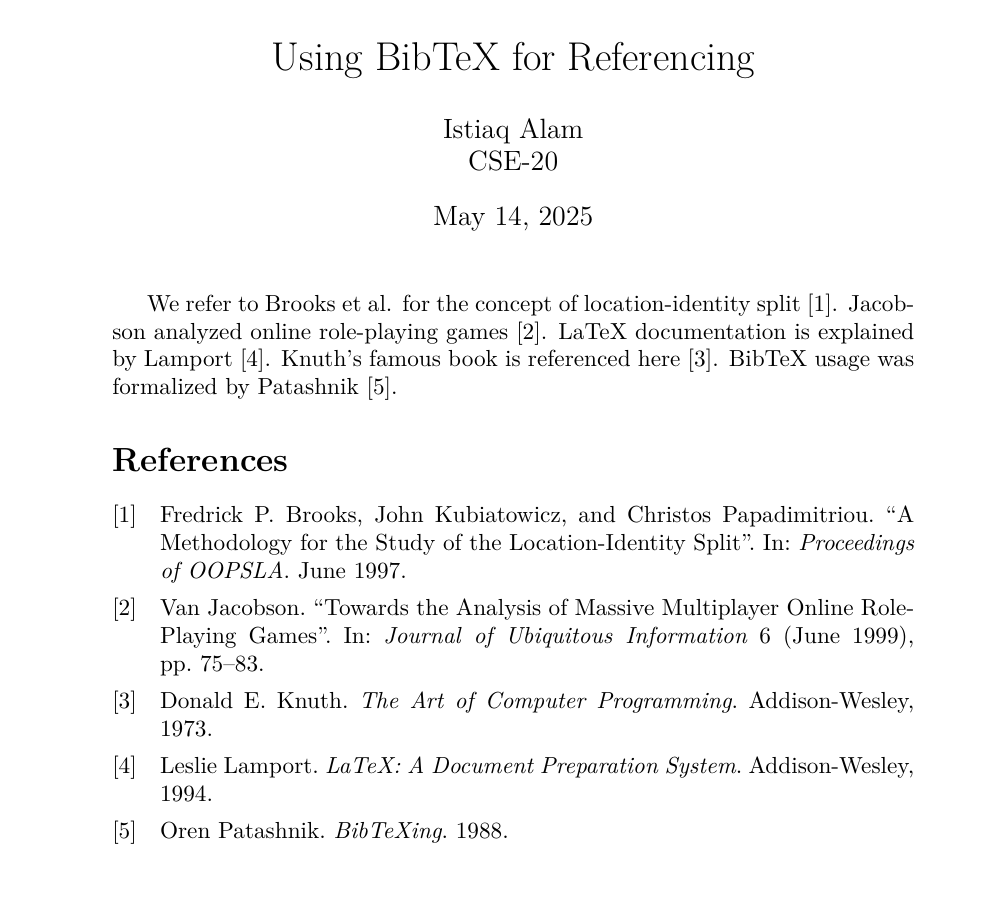
\includegraphics[width=0.9\textwidth]{lab8.png}
%\caption{\label{table}Output of the Article}
\end{figure}
\vspace{9em}
\begin{center}
\Huge THE END
\end{center} 
\end{document}